\chapter{Introduction to routing schemes}

Routing is one of the most fundamental problems in the area of distributed
networking. The goal in this problem is to find a distributed algorithm that
allows any source vertex $v$ in a network $G=(V,E,\omega)$ to route messages
to any destination vertex $u$, where $u, v\in V$.

Each node $v \in V$ is given a unique name with $O(log\; n)$ bits. Also,
for each vertex, each outgoing edge is given a unique port number in
$\{1,\dots,deg(v)\}$.

%Formally, a routing scheme is comprised of two phases. The first phase is
%called the preprocessing phase. In this phase $G$ is preprocessed and the
%derived routing information is stored locally with the relevant vertices.

%In the second phase - the routing phase - the routing scheme allows any vertex
%to route messages to any vertex in a distributed manner only based on the
%label of the destination vertex.

A naive approach to routing is to preprocess a graph by running a SSSP %single source ??
algorithm from each vertex $v \in V$ and at each vertex $v$ store a hashmap
mapping every vertex $u\in V$ to a port number of $v$, such that following this port will be the first edge of a shortest path to $u$ from $v$.

When routing, a vertex $v$ will only need to look at the destination label
of the message. If the destination label match $v$ we are done, otherwise we 
lookup the port for the destination vertex and forwarding the message via that port.

This approach will ensure a routing of stretch-1 (a min cost path) and the lookup performed at
each vertex can be done in constant time. But this approach will use a great amount of 
space as each vertex will store a hashmap with $n$ entries where each key is a
destination label using $O(log(n))$ bit.

Thus the space consumed at each node is $\Omega (n\; log\; n)$. This space
complexity renders our naive approach useless as it does not scale well.

In order to reduce memory usage and ensure for routing costs that are proportional
to distances, there are two parameters that routing schemes seek to minimize.
\begin{description}
  \item[Stretch] The max ratio over all source-destination pairs between the
      cost of the path taken by the routing scheme and the cost of a min
      cost path.
  \item[Memory] The max number of bits over all nodes stored for the routing
      scheme. (balanced is preferred)
\end{description}
This article presents a routing scheme that uses $\tilde{O}(\sqrt(n))$
routing table space per vertex, and routes along paths of stretch-3. Note that $\tilde{O}()$ abstracts away factors of logarithmic size, just like $O()$ abstracts away constants.

\section{Labeled Routing or Name-Independent Routing}
In the literature we distinguish between \emph{labeled routing} or
\emph{name-independent routing}. To illustrate the differences we look at a complete
grid and imagine that the intersections is vertices and the lines are edges, as seen in \autoref{fig:labeledrouting}.

In labeled routing we are allowed to label the vertices ourself. This allows
us to give every vertex a label representing the $(x,y)$-coordinate of that
vertex. This way we encode topological information into the label names and we
can easily navigate in the graph by forwarding messages to desired port. In
this scenario the available ports for each vertex would be a subset of $\{+y,
-y, +x, -x\}$.
\begin{figure}[htbp]
    \centering
    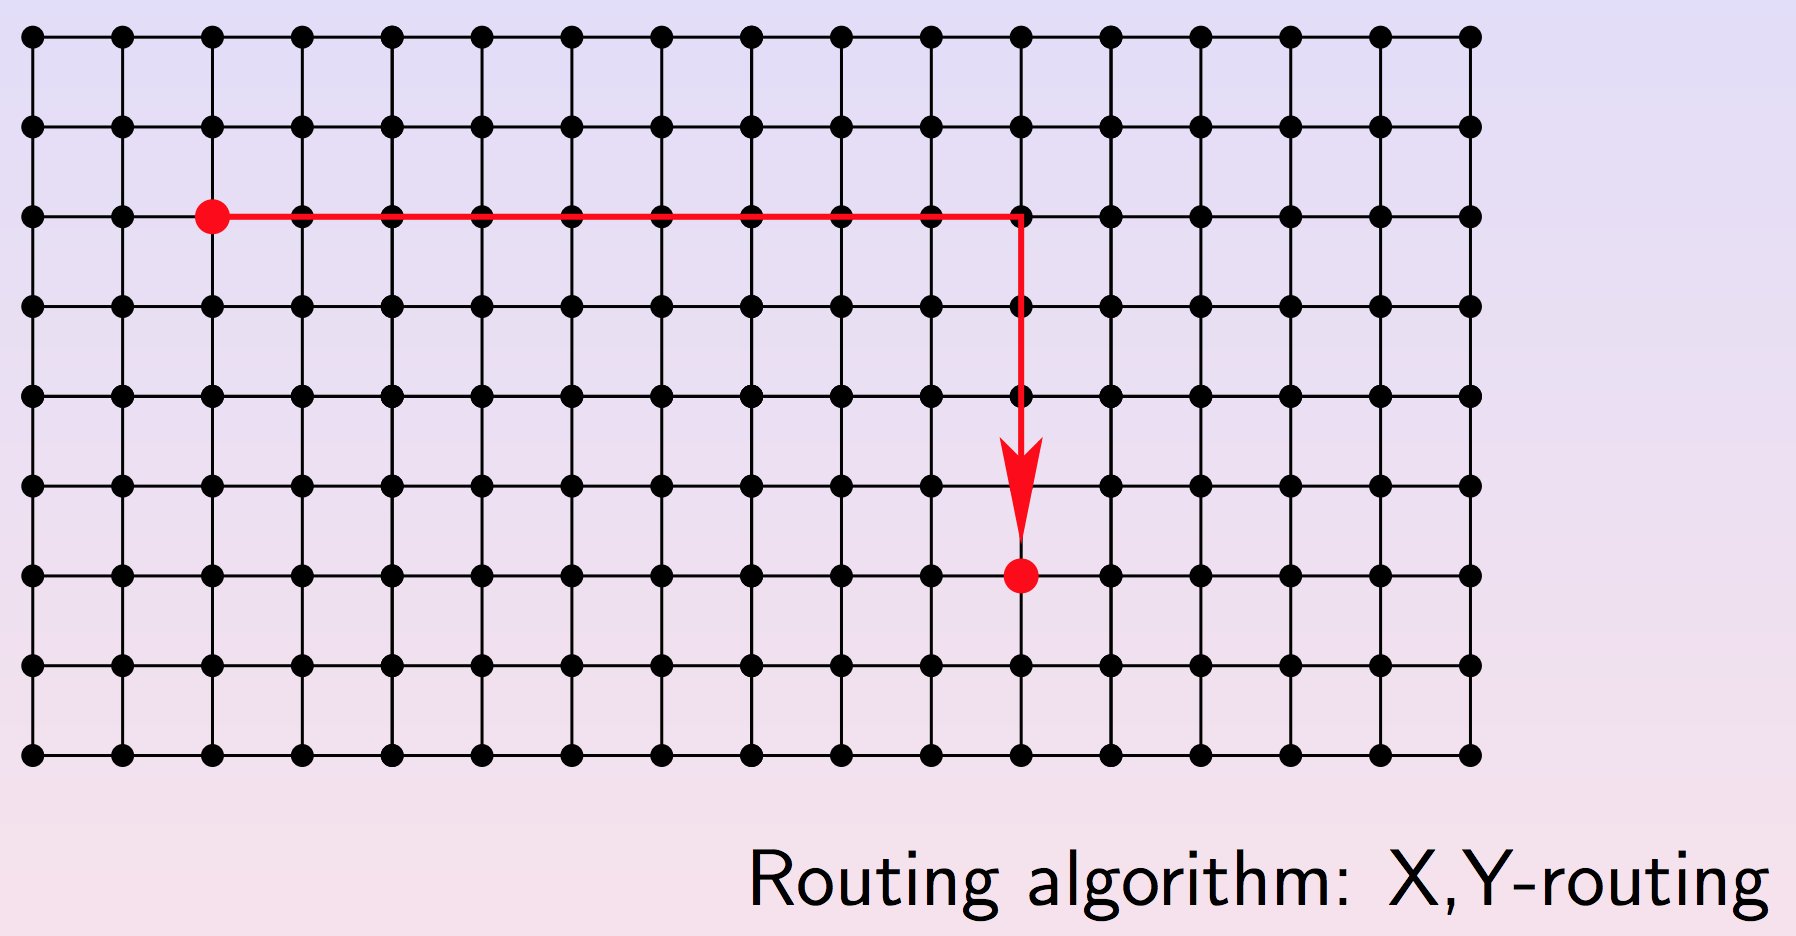
\includegraphics[scale=0.3]{images/xyrouting.png}
    \caption{x-y-routing}
    \label{fig:labeledrouting}
\end{figure}

In contrast, when doing name independent routing, an adversary will label the
vertices. If the labeling is done randomly it will hold no routing information
and we can't use the label names to navigate directly, as done in labeled routing. Thus, we need some kind of
technique to figure out what port to use for message forwarding at each vertex.

In this article we present a compact name-independent routing scheme with minimum stretch.
%TODO describe compactness

This scheme requires (uses) rewritable packet headers (which all previous name-independent schemes also do), as a scheme that does not rewrite packet headers must be loop free and thus must have a stretch of 1 on any tree. This however means that it cannot be compact, by Lemma 2.1 \cite{compactNameIndepRouting}[37:4]. A lower bound for compact labeled routing by Gavoille and Gengler [2001] \cite{gavoilleAndGengler2001} shows that any stretch $< 3$ scheme must use a total of $\Omega(n^2)$ bits. Thus it cannot be that all nodes use only $o(n)$ bits (at least one must use more. This bound also holds for name-independent routing. Actually, Gavoille and Gengler [2001] \cite{gavoilleAndGengler2001} imply that compact routing schemes with stretch 3 and requires at least $\Omega(\sqrt{n})$. bits per node.

%An even stronger memory bound of $\Omega(n^2\log\;n)$ bits for stretch $< 3 $ can be proven for the name-independent scheme. Lemma 2.2 \cite{compactNameIndepRouting}[37:4] shows that for at name-independent routing scheme with $o(n\;log\;n)$ bits per node must have stretch at least 3.

Thus it is known that no compact routing using $o(n)$ space per node can route with stretch below 3. The presented compact name-independent routing scheme is indeed with minimum stretch 3 using $\tilde{O}(\sqrt(n))$ bits per node.